\section{Results}
\subsection{\fred as a Teaching Aid}

\fred (v0.0.3)\cite{stephen_thompson_2020_3946090} was used at our Medical Summer School in 2020 with a cohort of 5 students. Feedback suggested that it had improved their understanding
of fiducial based registration. 

\subsection{Extension to Anisotropic Errors}
We simulated an anisotropic independent \gls{FLE}, with \gls{FLE} in the x 
direction being 3 times that in the y and z, as described in Section \ref{sec:anis_method}.
Errors were scaled so that the 
expected absolute value of the \gls{FLE} was the same as for the isotropic case. 
\fred was then used to perform at least 200 simulated registrations, the results of
which are shown in Fig. \ref{fig:anis_error}. 

\begin{figure}
	\begin{center}
			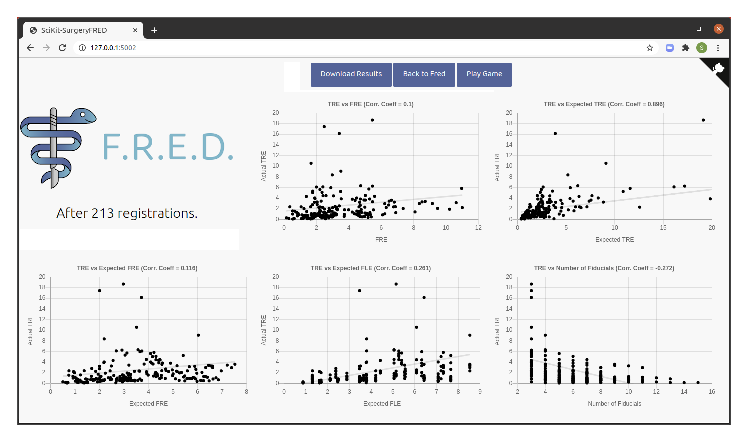
\includegraphics[width=0.9\linewidth]{images/anisitropic_error.eps}
		\caption{\label{fig:anis_error}Results of over 200 registrations using an anisotropic model of {FLE}}
	\end{center}
\end{figure}

It was apparent when preforming the registrations that the majority of target 
registration error was in the x direction. However this is not communicated in the 
statistics of Figure \ref{fig:anis_error}. It would be an interesting extension 
exercise to use \fred to explore ways of communicating anisotropic errors during 
treatment.

\subsection{Addition of Systematic Errors}
We added a systematic \gls{FLE} as an isotropic uniform random variable, in the range
-0.5 to 0.5, as described in Section \ref{sec:sys_method}. This error will be applied to all fiducial markers for a 
given registration. We performed at least 200 simulated registrations using \fred, the results of which are shown in Fig. \ref{fig:sys_error}.
\begin{figure}
	\begin{center}
			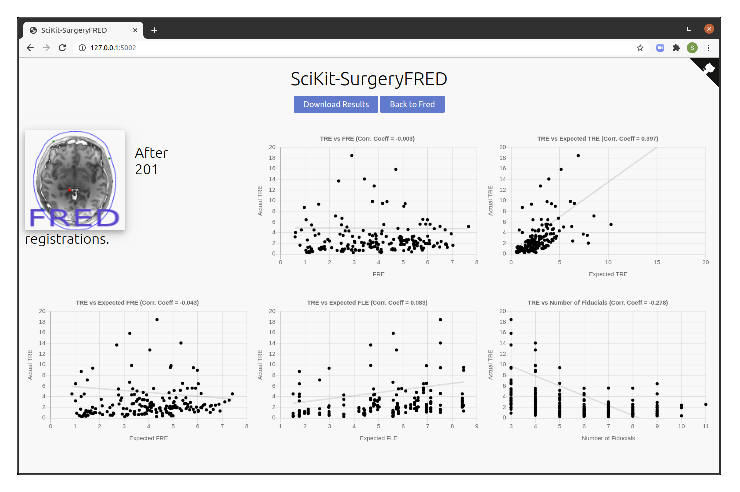
\includegraphics[width=0.9\linewidth]{images/systematic_error.eps}
			\caption{\label{fig:sys_error}Results of over 200 registrations with systematic error.}
	\end{center}
\end{figure}

It is noticeable that average \gls{TRE}s are higher than in cases where there is no
systematic error, while \gls{FRE} remains similar. This is as expected as \gls{FRE} will 
not account for systematic errors. This is a useful demonstration of this effect, though 
it might be more instructive to implement systematic errors in the game based method, see
Section \ref{sec:game_method}, to investigate the likely clinical impact of these
systematic errors.

\subsection{\fred for Research in System Usability}
The results of the game based usability study are shown in Figure \ref{fig:usability}. As expected scores are 
highest when the actual \gls{TRE} is known. Interestingly it appears that when told only the expected value of the \gls{FLE} the students
tended to under treat the target more, resulting in lower overall scores. This study currently only has 100 data points (20 for each category)
so it must be stated that the results are not yet statistically significant. 

\begin{figure}
        \begin{center}
        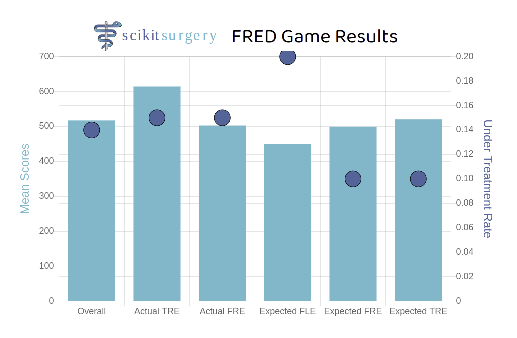
\includegraphics[width=0.5\linewidth]{usability.eps}
                \caption{\label{fig:usability}Average scores and treatment failure rates for the game based usability study.}
	\end{center}
\end{figure}



